 47675896 i\chapter[Metodolog\'ia.]{Metodologia}
\pagestyle{fancy}

En este cap\'itulo se describen las consideraciones tenidas en cuenta para el desarrollo de la sonda, el diseño mec\'anico, el\'ectrico, electr\'onico, control y comunicaci\'on de cada uno de los componentes que componen la sonda y su sistema de despliegue. Adem\'as de los diagramas, algoritmos de funcionamiento y el caso de aplicaci\'on en el PINV15-177.

\section[Consideraciones del sistema]{Consideraciones de Dise\~no}
Para el desarrollo de la soluci\'on presentada, se tuvo en cuenta las siguientes consideraciones:
\begin{itemize}
    \item Portabilidad: Se espera que la sonda sea transportable por una persona sin mucho problema, el di\'ametro debe ser menor a 150[mm].
    \item Asequibilidad: Se espera que el costo final pueda ser reducido menor al 20\% del costo de una soluci\'on comercial parecida(Libelium Smart Water Xtreme), valorada en \$ 11.200 (once mil doscientos d\'olares americanos) \cite{storeLibelium}, sin contar los impuestos y gastos de importaci\'on.  
    \item Escalable: Se espera que la soluci\'on pueda ser escalable y configurable, seg\'un la necesidad. Vers\'atil para que pueda ser compatible con otros sensores con peque\~nos o ningún cambio en la sonda.
    \item Compatibilidad: Se espera que la sonda pueda ser compatibles con varios protocolos de comuncic\'on y con otros sensores, con la menor cantidad de adaptaciones mec\'anicas o electr\'onicas. 
    \item Rangos de medici\'on: Considerando que el lugar de despliegue de la sonda, ser\'a en el lago Ypakarai, se espera que la soluci\'on pueda desenvolverse sin problemas hasta 4 metros de profundidad, considerando el estudio de batimetr\'ia realizado por el laboratorio de Soluciones tecnol\'ogicas para la gesti\'on Integral de los Recursos H\'idricos. Anexo \ref{fig:BatimetriaItaipu}
    \item Adaptable: Se espera que la soluci\'on pueda ser utilizado con diferentes sistemas de despliegue.
    \item Open Source: Se espera que durante el desarrollo de la soluci\'on se prioricen los sistemas open source para reducir costos y poder contribuir al ecosistema. 
    \item Autonom\'ia: Se espera que la soluci\'on presentada se pueda utilizar sin necesidad de estar sujeto a otros sistemas y que cuenta con una fuente de alimentaci\'on independiente y recargable para permitir muestro de hasta por lo menos 10 horas continuas, que es la duraci\'on promedio de luz natural \cite{ClimaSol}. 
    
\end{itemize}

Teniendo en cuenta las consideraciones y criterios antes expuestas y luego de la revisi\'on de los trabajos de otros autores, estudiados en el cap\'itulo anterior. A continuaci\'on se abordar\'a el proceso de desarrollo involucrado, a modo de orden se dividi\'o todo el proceso en tres grandes secciones, los cuales son Disen\~no, en el cual se detallan los planos y diagramas m\'ecanicos de cada uno de los elementos del sistema en la subsecci\'on de dise\~nos m\'ecanico, los diagramas, planos y esquemas de conexi\'on el\'ectrica en la subsecci\'on de dise\~no el\'ectrico, en la subsecci\'on de dise\~no electr\'onico se abarcara lo concerniente al diseño electr\'onico circuitos de adquisici\'on de datos de los sensores, drivers y otros elementos, en la subsecci\'on de la base de datos y control. 

\section{Dise\~no}

\subsection[Dise\~no M\'ecanico]{Dise\~no M\'ecanico}
\subsubsection[Sonda]{Sonda}

El dise\~no final fue un proceso evolutivo resultado de varias iteraciones y resultado de procesos evolutivos iniciado en el proyecto Cormor\'an-I detallado en el anexo \ref{Anexo:Cormoran},  partiendo el modelo utilizado por Hitz y otros\cite{hitz2012design}, %% Colocar Graficos o referenciar del cap2

hasta la versi\'on final, aunque esta soluci\'on est\'a pensada principalmente para el proyecto PIN15-177, la idea tras este trabajo es adem\'as, contar con un dispositivo capaz de funcionar de forma independiente a cualquier otro tipo de veh\'iculo, extendiendo as\'i sus posibles tipos de usos, como el monitoreo de acu\'iferos, esto supone que la sonda deba contar con todos los elementos necesarios para su correcto desenvolvimiento, la funci\'on principal de la sonda es brindar soporte a cada uno de los sensores, el soporte incluye el procesamiento de se\~nal, alimentaci\'on, almacenamiento de datos, protecci\'on contra impactos y transmisi\'on a una estaci\'on base remota los datos sensados.

Para el proyecto PIN15-177, la sonda a ser implementada debe de dar soportes a inicialmente cinco sensores (ph,CE,OD,OPR,T) y el dise\~no debe soportar la incorporaci\'on y/o retiro de alg\'un sensor, sin que esto conlleve adaptaciones importantes en la sonda, por ese motivo se opt\'o por un dise\~no modular de tal forma que, cuando sea necesario modificar alg\'un sensor se tenga que reemplazar simplemente uno de los m\'odulos y de esta forma reducir los costos. Los tres mo\'dulos est\'an compuestos por:
\begin{itemize}
    \item \textbf{Frente}: Este m\'odulo es la pieza frontal de la sonda, cuya funci\'on principal es de protecci\'on a cada uno de los sensores contra basuras u objetos con que puede entrar en contacto directo y adem\'as de crear un entorno de volumen de agua constante y reducir en la mayor medida posible la formaci\'on de turbulencias alrededor de los sensores para evitar los fallos o errores de lecturas de los sensores que se podr\'ian registrar a causas de burbujas de aire en los cabezales de los sensores. Tal como indica en la figura \ref{fig:Frente}, la zona comprendida dentro del recuadro rojo. As\'i como se indica en el plano del anexo \ref{fig:ModuloFrontal}, para el dise\~no de est\'e m\'odulo, se parti\'o de una forma cil\'indrica hueco de altura suficiente para poder cubrir totalmente cada uno de los sensores, con aberturas longitudinales equidistantes en las paredes laterales en forma de ranuras con bordes redondeados, una de las bases totalmente libre para que se pueda acoplar a los otros m\'odulos y  la otra base redondeado de forma esf\'eorico hueco, a fin favorecer el efecto hidrodin\'amico al momento del contacto con el agua, como se presentara m\'as adelante con las simulaciones realizadas.
    
    \begin{figure}[H]
        \centering
        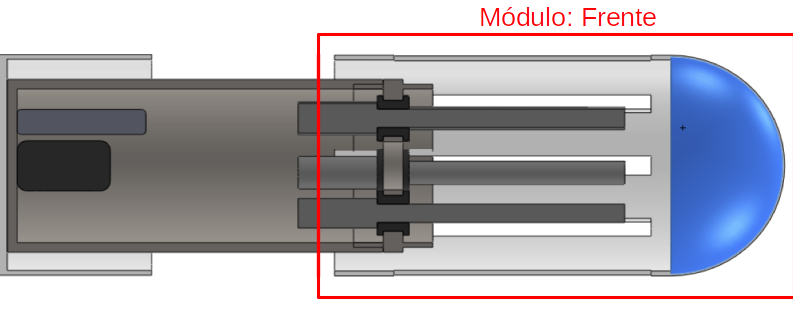
\includegraphics[width=110mm, height=40mm]{Imagenes/cap3/CompletoV5_Frente.png}
        \caption[Corte Transversal]{Corte Transversal Sonda. M\'odulo: Frente.}\textbf{Fuente:} Elaboración Propia.
        \label{fig:Frente}
    \end{figure}
    \item \textbf{Base}: Este m\'odulo, es la parte posterior de la sonda, su función principal es de almacenar de forma segura todo el equipamiento electr\'onico de control, el\'ectrico, almentaci\'on y placas necesarias para los sensores, tal como se indica en la figura \ref{fig:Base2020}, la base est\'a conformada por un cilindro hueco de 270 [mm] de altura, 120[mm] de di\'ametro exterior, espesor de las paredes internas laterales de 10[mm] y un espesor de la base 15[mm],  para sellar de forma herm\'etica, se utilizó un roscado Whitworth fino, utilizada para tuber\'ias de gas y de agua\cite{falk_metalotecnia_1986}, de paso 1,154 [mm].
    
    \begin{figure}[h]
    \centering
    \fbox{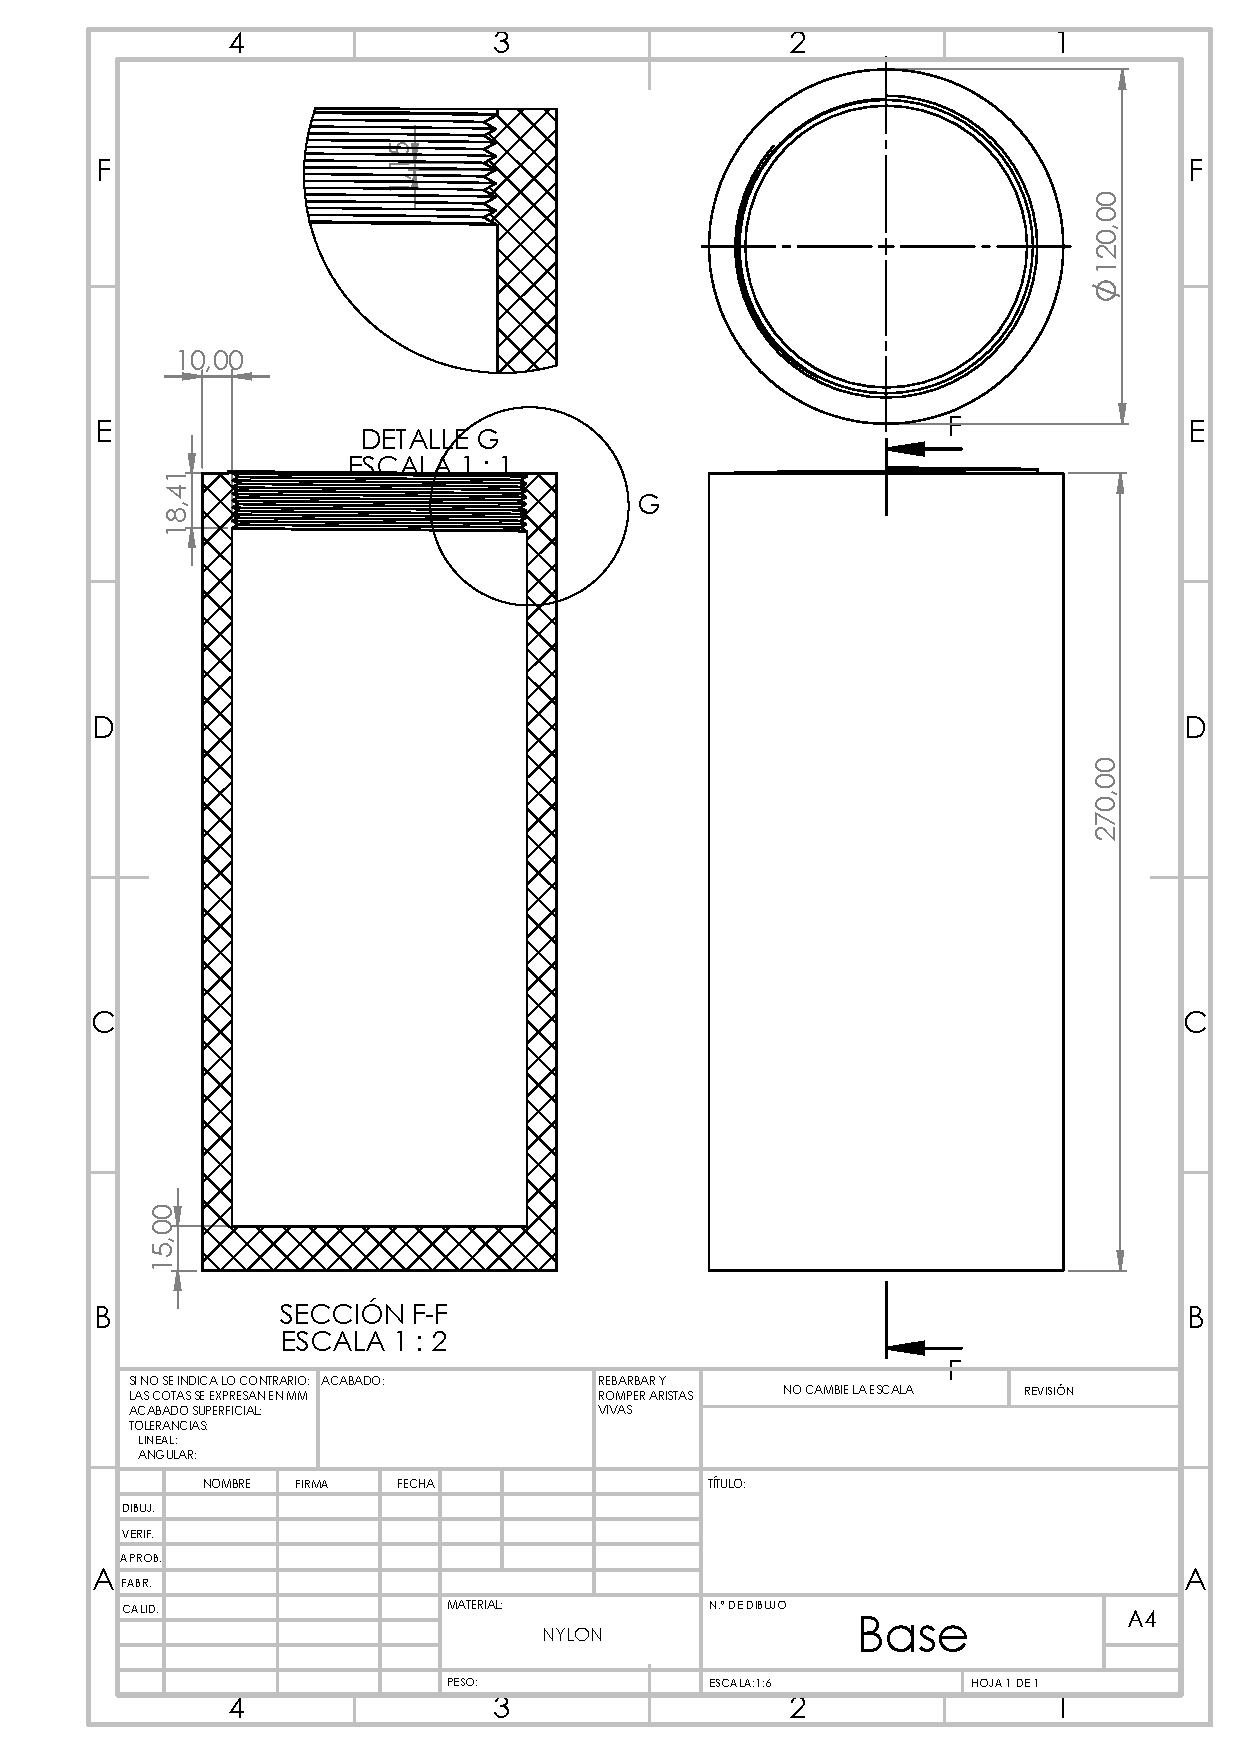
\includegraphics[scale=0.45]{Imagenes/2019/Base2019.PDF} }
    \caption{Dise\~no final de la base. \textbf{Fuente}: Elaboraci\'on propia}
    \label{fig:Base2020}
    \end{figure}
    \item \textbf{Anillo}: Tercer m\'odulo, es la parte centrar de la sonda, adem\'as de servir como enlace entre las otras dos piezas, tiene dos funciones principales, en primer lugar acoplarse a la base cerr\'andolo de forma herm\'etica y la segunda de sostener los sensores en sus posiciones fijas en la sonda. Este es el m\'odulo m\'as peque\~no en relaci\'on a las otras dos, se dise\~no de esta forma para ser el \'unico m\'odulo que se espera se tenga que reemplazar en el caso de ser necesario una reconfiguraci\'on u modificaci\'on de los sensores. Tal como se muestra en la figura \ref{fig:Anillo2019} el dise\~no parte de un cilindro macizo de 70 [mm] de altura y 120[mm] de di\'ametro exterior, se utiliz\'o Whitworth fino al igual que la base a fin de que pueda enroscarse  perfectamente, con el roscado se asegura hasta cierto punto el cierre herm\'etico entre los dos m\'odulos, como medida de seguridad extra se introducen los o-ring, para crear otro  sello hermético al momento del contacto entre las dos m\'odulos, con estos dos sistemas se espera que el ingreso de l\'iquidos sea nulo o m\'inimo, para la implementaci\'on de la sonda en este trabajo se utilizaran 5 sensores, y como esta secci\'on es la encargada que mantener en su posici\'on cada uno de los sensores, se realizan cinco perforaciones en este m\'odulo a fin de poder colocarlos de forma perpendicular. Como estas perforaciones para los sensores implicar\'ia posibles en \'areas de ingreso de l\'iquido, considerando adem\'as que el uso de o-ring se tornan un poco complicados para la posterior fabricaci\'on, se opt\'o por utilizar juntas hidr\'aulicas estandarizadas con el di\'ametro interno compatible con el di\'ametro del los sensores, dispuesta en pares por cada uno de los sensores a fin de 
    
    \begin{figure}[h]
    \centering
    \fbox{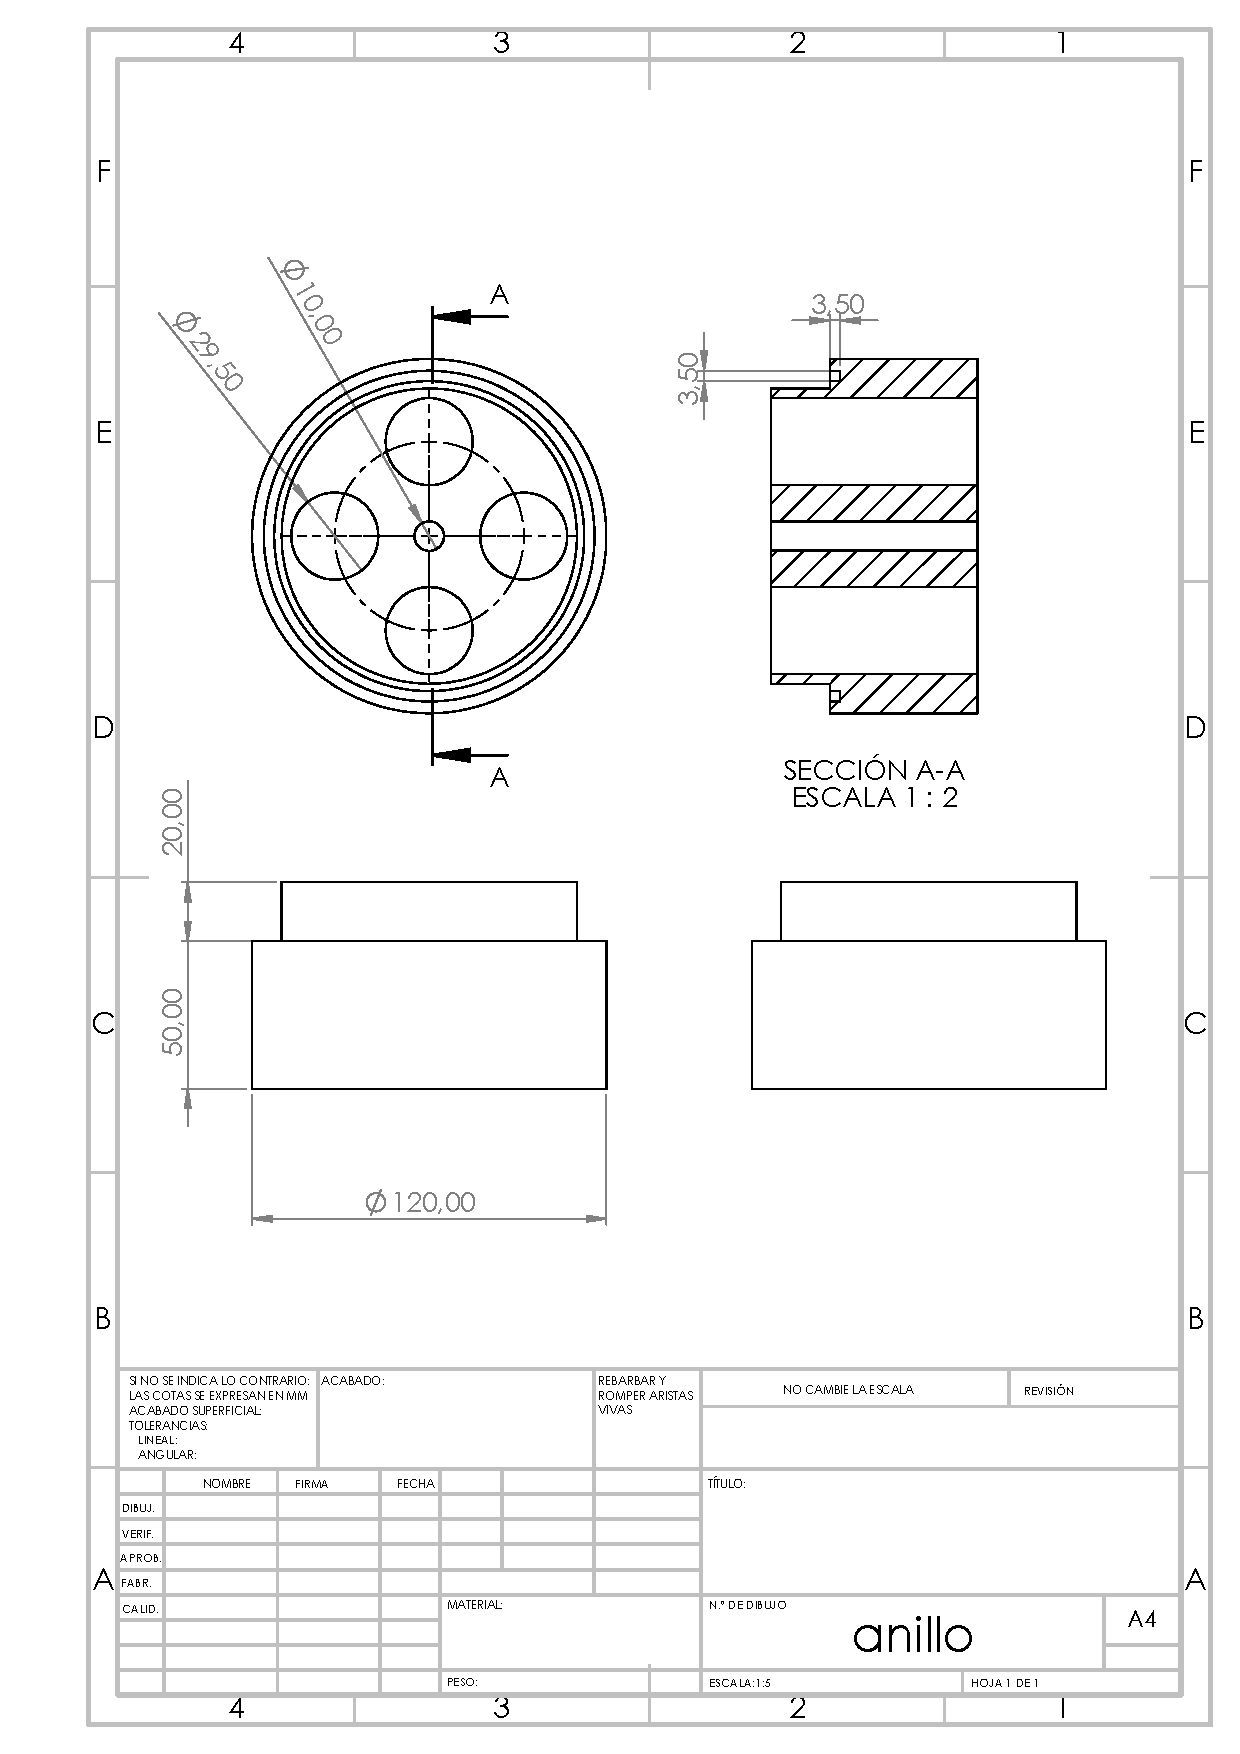
\includegraphics[scale=0.6]{Imagenes/2019/anillo2019.PDF} }
    \caption{Dise\~no final del anillo. Fuente: elaboración propia}
    \label{fig:Anillo2019}
    \end{figure}
\end{itemize}

\subsubsection[Batimetr\'ia]{Batimetr\'ia}
Este subsistema auxiliar, está pensado por la capacidad de medici\'on a multi niveles, cuando se requiera que la sonda descienda el subsistema se encargara de censar la profundidad en el punto de descenso y mandar la informaci\'on a la sonda para seteo de la carrera de la gr\'ua. Se opt\'o por una estructura simple, de bajo costo,  modular y vers\'atil para varios modos de uso.  
La estructura est\'a compuesta por

\subsubsection[Gr\'ua ]{Gr\'ua}


\subsection[Dise\~no El\'ectrico]{Dise\~no El\'ectrico}
\subsubsection[Sonda]{Sonda}
Para lograr autonom\'ia energ\'etica para la sonda se opto por utilizar bater\'ias LiPo Nano-Tech por sus caracter\'isticas t\'ecnicas que permitir\'an alimentar de forma suficiente a toda los componentes que conforman la sonda, como se aprecia en la Figura \ref{fig:4.17}. 

Las baterias Turnigy nano-tech Lipoly bater\'ias fueron dise\~nados para alto rendimiento . Utilizando un avanzado sustrato electrones que permite pasar m\'as libremente de \'anodo a c\'atodo con menos impedancia interna.
 Las ventajas que presenta la utilización de esta fuente son la posibilidad de tener tensiones de +/- 3.3V, +/-5V y +/-12V sin la necesidad de realizar circuitos para la obtención de estos voltajes en comparación a la utilización de baterías de litio.
 \newline
 \hfill
Las ventajas sobre las bater\'ias tradicionales LIPOLY;
\begin{itemize}
    \item La densidad de potencia alcanza 7,5 kW / kg.
    \item Menos hueco de tensi\'on durante la descarga de alta velocidad, dando m\'as poder bajo carga.
    \item Impedancia interna puede llegar tan bajo como 1.2 m${\Omega }$ en comparación con la de 3 m${\Omega }$ de un Lipoly estándar
    \item Control t\'ermico m\'as, paquete por lo general no supera 60 $^{\circ}$C.
    \item Hinchazón durante la carga pesada no supera 5\%, en comparación con 15\% de un Lipoly normal.
    \item Mayor capacidad durante la descarga pesada. M\'as del 90\% a la tasa de 10O\% C.
    \item Carga r\'apida capaz, hasta 15$^{\circ}$C en algunas baterías.
    \item Mayor duraci\'on del ciclo, casi el doble que el de la tecnolog\'ia LiPoly est\'andar.
\end{itemize}


La tecnolog\'ia de nano-core en las bater\'ias de litio es la aplicaci\'on de aditivos conductores nan\'ometros. Los aditivos nan\'ometros conductora forman redes ultra-fuertes de electrones de conducci\'on en los electrodos que pueden aumentar la conductividad electr\'onica.

Estos aditivos crean la capacidad de imbibici\'on en el l\'iquido portador para suministrar m\'as canales de iones. Esto mejora la capacidad de transmisi\'on de iones y la difusi\'on de iones. A trav\'es de la mejora de la conductividad y de iones de transmisi\'on electr\'onica, la impedancia se reduce y la polarizaci\'on de la descarga de alta tasa disminuye en gran medida.

\hfill
\begin{table}[t]
\protect\caption[Caracter\'isticas de bater\'ia Lipo Nano-Tech ]{Caracter\'isticas de bater\'ia Lipo Nano-Tec 5100mAh.}
\label{tab:caract_bat}
\begin{center}
\begin{tabular}{|l|l|}
\hline
Capacidad    &  5100 mAh \\
\hline
Voltaje      &  2S3P/ 7.4 V \\
\hline
Descarga &  65C / 135C \\
\hline
Peso  & 290 g\\
\hline
Dimensi\'on   &  69x47x25 mm\\
\hline
Conector equilibrio	& JST\\
\hline
\end{tabular}
\vspace{5mm}
\newline
\hfill \textbf{Fuente:} P\'agina Web del Fabricante\cite{bateria}
\end{center}
\end{table}

En contrapartida, limitará a nuestro sistema, ya que deberá ir conectado a la red eléctrica todo el tiempo que se requiera del uso de la misma.
\section[Características Técnicas de los módulos]{Características Técnicas del módulo Sonda}
La Tabla \ref{tab:carac_general} detalla las características técnicas del mecanismo a ser desarrollado, teniendo en cuenta los objetivos planteados en la Sección 1.3.

\begin{table}[H]
\protect\caption[Datos Técnicos]{Datos Técnicos. \label{tab:carac_general}}
    \centering
    \scalebox{0.9}{\begin{tabular}{|c|c|}
        \hline
        \textbf{Característica} & \textbf{Valor}  \\
        \hline
        \multicolumn{2}{|c|}{\textbf{Sensores}} \\
        \hline
        Cantidad & $ 5 $   \\
        \hline
        \multicolumn{2}{|c|}{\textbf{Físico}} \\
        \hline
        Dimensiones & $< 50 [cm]$  $< \phi 15[cm]$   \\
        \hline
        Peso &  $ > 6 kg$ \\
        \hline
        Caja Electrónica & Herm\'etica  \\
        \hline
        \multicolumn{2}{|c|}{\textbf{Eléctrico}} \\
        \hline
         Alimentación & 5 V DC  \\
        \hline
         Autonomía & LiPo 5100mAh  \\
        \hline
         \multicolumn{2}{|c|}{\textbf{Interfaz}} \\
         \hline
         Configuración de Parámetros & Por Interfaz Gráfica, SSH, VNC  \\
        \hline
         Transmisi\'on Remota  & Si  \\
        \hline
    \end{tabular}}
    \vspace{5mm}
    \newline
    \hfill \textbf{Fuente:} Elaboración Propia
\end{table}

\subsubsection[Batimetr\'ia]{Batimetr\'ia}
\subsubsection[Gr\'ua ]{Gr\'ua}


\subsection[Dise\~no Electr\'onico]{Dise\~no Electr\'onico}
\subsubsection[Sonda]{Sonda}
\paragraph[Interfaz de Sensores]{Interfaz de Sensores}
Es el bloque donde se obtiene las mediciones de las caracter\'isticas f\'isico - qu\'imica del recurso h\'idrica, para su posterior procesamiento, almacenamiento y transmici\'on a base remoto.

\subparagraph{Sensor de pH}
En la Figura \ref{fig:4.8} se puede apreciar el sensor de pH por el que se optó fabricado por la empresa Atlas Scientfic.
    \begin{figure}[t]
    \centering
	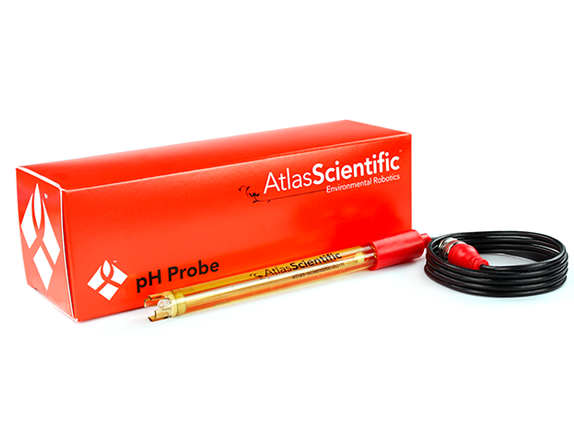
\includegraphics[width=150mm, height=90mm]{Imagenes/2021/imag23.png}%\textwidth%
	\caption[Sonda de pH de la empresa Atlas Scientific]{Sonda de pH de la empresa Atlas Scientific. \textbf{Fuente:} Página Web del fabricante.}
	\label{fig:4.8}
    \end{figure}
Los criterios para la selección de este sensor fueron, su simplicidad de uso gracias a su extensa documentación y soporte por parte del fabricante, su popularidad en el ámbito de la automatización y control de calidad de agua para varios tipos de usos y su integración dentro de la placa de desarrollo sin necesidad de cableados externos y compatible con el módulo EZO pH Circuit que se muestra en la Figura \ref{fig:4.9}
\newline
\hfill
    \begin{figure}[H]
    \centering
	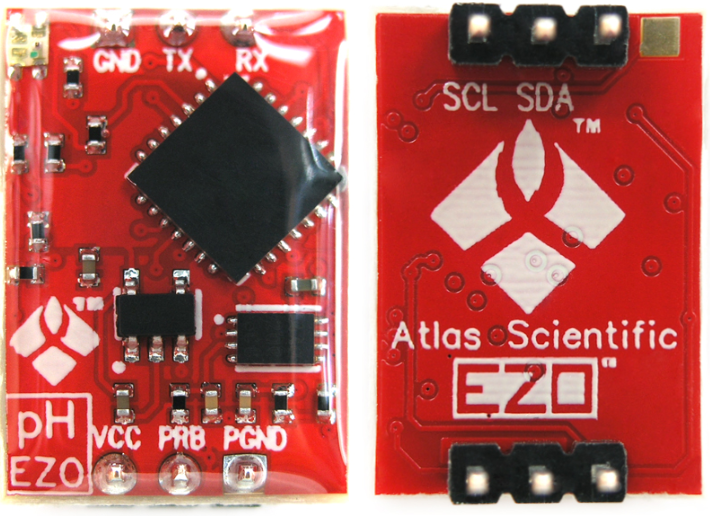
\includegraphics[width=70mm, height=60mm]{Imagenes/2021/imag27.png}%\textwidth%
	\caption[EZO pH Circuit]{EZO pH Circuit.\textbf{Fuente:} Pagina Web del Fabricante.}
	\label{fig:4.9}
    \end{figure}
El módulo es un dispositivo bastante sensible, y ésta sensibilidad es lo que le da una excelente precisión. Significa que es capaz de leer microvoltajes que están presentes en el agua de fuentes no naturales como bombas, válvulas de solenoide u otras sondas o sensores lo que ocasiona lecturas que fluctúan rápidamente o lecturas que están constantemente apagadas.

Al leer el pH y la conductividad u oxígeno disuelto juntos, el fabricante recomienda que los módulos estén aislados eléctricamente de los demás circuitos, subsanados con el la placa de Tentacle.
\newline
\hfill
\begin{figure}[t]
    \centering
    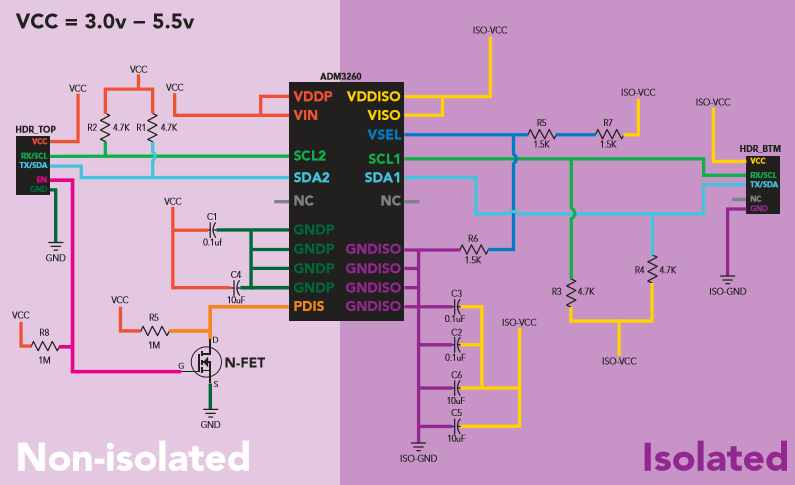
\includegraphics[width=150mm, height=90mm]{Imagenes/2021/imag36.png}
    \caption[Esquema de Funcionamiento del circuito EZO pH]{Esquema de Funcionamiento del circuito EZO pH.\textbf{Fuente: }Pagina Web del Fabricante\cite{ezoph}.}
    \label{fig:4.10}
\end{figure}
En la Figura \ref{fig:4.10} se muestra  el esquema del circuito interno del módulo, cómo están aislados datos y la potencia con el ADM3260, que es el chip encargado de realizar la aislación de los canales I2C utilizados y algunos componentes pasivos. El ADM3260 puede generar una potencia aislada de hasta 150 mW e incorpora dos canales de datos bidireccionales.
Esta tecnología funciona mediante el uso de pequeños transformadores para inducir el voltaje a través de un espacio de aire. Los dos canales de datos tienen una resistencia de extracción de 4.7 k$\Omega$ tanto en las líneas aisladas como en las no aisladas (R1, R2, R3 y R4). El voltaje de salida se configura mediante un divisor de voltaje (R5, R6 y R, 7). produce un voltaje de 3.9V independientemente de su voltaje de entrada.


\textbf{Principio de Operación: }Una sonda de pH mide la actividad del ion de hidrógeno en un líquido, en el extremo inferior de ésta hay una membrana de vidrio que permite a los iones de hidrógeno del líquido que se está midiendo depositarse en la capa exterior del vidrio, mientras que los iones más grandes permanecen en la solución. En la Figura \ref{fig:4.11} se pude apreciar el comportamiento de los iones de hidrógeno de acuerdo al tipo de solución que se tiene. La diferencia en la concentración de iones de hidrógeno (fuera de la sonda y en el interior de la sonda) crea una corriente muy pequeña. Esta corriente es proporcional a la concentración de iones de hidrógeno en el líquido que se mide.
La corriente que se genera a partir de la actividad del ion hidrógeno es el recíproco de esa actividad y se puede predecir usando esta ecuación:
\begin{equation}
E=E^0 + \frac{RT}{F}\times \ln\alpha_{H+} = E^0 - \frac{2.303RT}{F}\rho H
\label{eq:iv}
\end{equation}
Donde $R$ es la constante ideal del gas, $T$ es la temperatura en grados Kelvin y $F$ es la constante de Faraday.
\newline
\hfill
\begin{figure}[t]
\centering
	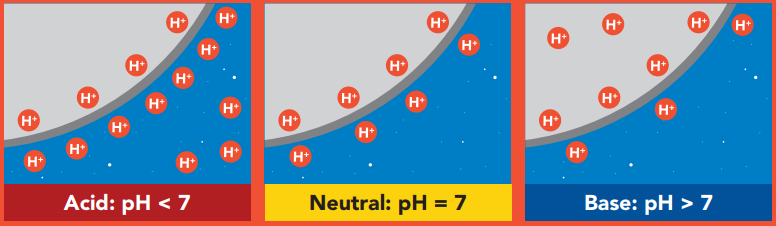
\includegraphics[width=160mm, height=70mm]{Imagenes/2021/imag22.png}%\textwidth%
	\caption[Actividad de los iones de hidrógeno]{Actividad de los iones de hidrógeno.  \textbf{Fuente:}Pagina Web del Fabricante \cite{atlasph}}
	\label{fig:4.11}
\end{figure}

En la Tabla \ref{tab: caract_sondaph} se detallan las características del sensor de pH.
\newline
\hfill
Entre las aplicaciones típicas en las que se utiliza esta sonda están, uso estándar de laboratorio, uso en el campo, en el suelo, cultivos con técnicas de hidroponía o acuaponía, muestras que contienen metales pesados,cerveza, vino y otros.

\begin{table}[H]
\protect\caption[Características del sensor de pH de AtlasScientific]{Características del sensor de pH de AtlasScientific.}
\label{tab: caract_sondaph}
\begin{center}
\begin{tabular}{|l|l|}
\hline
Rango    &  0 - 14\\
\hline
Exactitud      &  +/-0.002\\
\hline
Conector &  BNC macho\\
\hline
Resolución   &  +/-0.0001\\
\hline
Tiempo de Respuesta   &  95\% en 1s\\
\hline
Presión Máxima    &  100PSI\\
\hline
Profundidad Máxima	& 60m\\
\hline
Rango de Temperatura $^{\circ}$C	& 1- 99\\
\hline
Longitud del Cable	& 1m\\
\hline
Sensor de Temperatura Interno	& NO\\
\hline
Tiempo antes de recalibración	& 1 año\\
\hline
Tiempo de Vida	& aprox. 2.5 años\\
\hline
Seguro en Alimentos & Si\\
\hline
Peso & 49 gramos\\
\hline
Dimensiones & 12mm x 150 mm\\
\hline
\end{tabular}
\vspace{5mm}
\newline
\hfill
\textbf{Fuente: }Pagina Web del Fabricante\cite{atlasph}
\end{center}
\end{table} 


\subparagraph{Sensor de Conductividad}
El sensor utilizado para las lecturas de conductividad se puede apreciar en la Figura \ref{fig:4.12}, también de la empresa Atlas Scientific.
\begin{figure}[t]
\centering
	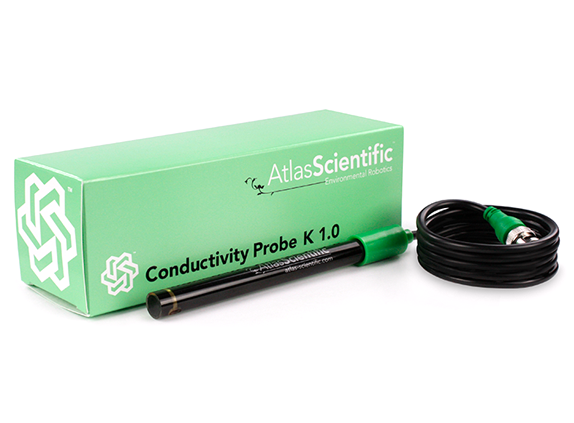
\includegraphics[width=150mm, height=90mm]{Imagenes/2021/imag24.png}%\textwidth%
	\caption[Sensor de CE]{Sensor de CE.  \textbf{Fuente:}Pagina Web del Fabricante \cite{atlasce}}
	\label{fig:4.12}
\end{figure}
Los criterios de selección fueron su extendido uso para control de calidad de aguas para varios usos, buen soporte y extensa documentación disponible en la web, la homogeneidad en los dispositivos electrónicos, al utilizar sensores ya compatibles (Sensor de pH y Sensor de CE) y con los debidos aislamientos requeridos entre estos.  
 
El módulo EZO conductivity Circuit, se muestra en la Figura \ref{fig:4.13} emplea un método de resolución de escala. A medida que aumenta la conductividad, la resolución entre lecturas disminuye como se puede apreciar en la Tabla \ref{tab:resol_ce}.
\begin{figure}[b]
    \centering
    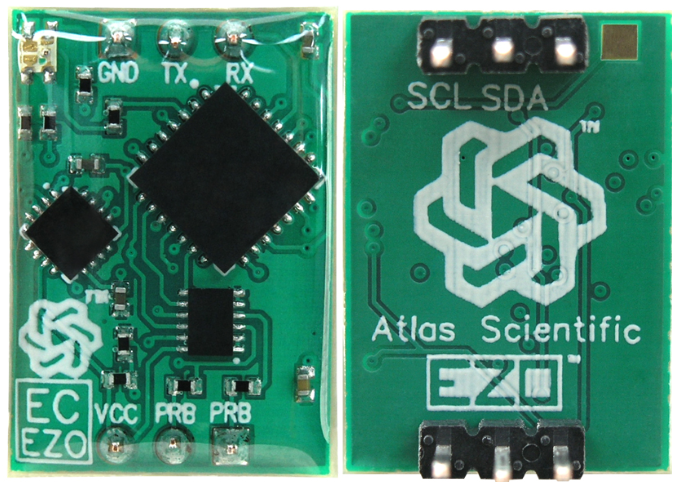
\includegraphics[width=70mm, height=60mm]{Imagenes/2021/imag28.png}
    \caption[EZO conductivity Circuit]{EZO conductivity Circuit. \textbf{Fuente: }Página Web del Fabricante.}
    \label{fig:4.13}
\end{figure}
El módulo emitirá lecturas de conductividad donde los primeros 4 dígitos son válidos y los demás se establecen en 0. Esto excluye las lecturas de conductividad que son menores a 9.99. En ese caso, solo se emitirán 3 dígitos de conductividad.

\begin{table}[t]
    \protect\caption[Resolución de Escala Sensor de Conductividad]{Resolución de Escala Sensor de Conductividad.}
    \label{tab:resol_ce}
    \centering
    \begin{tabular}{ c c }
         \toprule
         \textbf{Valor}&\textbf{Resolución}  \\
         \midrule
%         \hline
         0.07-99.99 & 0.01$ \mu S/cm$ \\
%         \hline
         100.1-999.9 & 0.1 $\mu S/cm $\\
%         \hline
         1,000-9,999 & 1.0 $\mu S/cm$ \\
%         \hline
         10,000-99,990 & 10.0 $\mu S/cm $\\
%         \hline
         100,000-999,99 & 100 $\mu S/cm$ \\
%         \hline
        \bottomrule
    \end{tabular}
   \vspace{5mm}
   \newline
   \hfill \textbf{Fuente: }\cite{ezoce}.
\end{table}

\textbf{Principio de operación: }
Una sonda de conductividad eléctrica (CE) mide la conductividad eléctrica en una solución. Se usa comúnmente en ecosistemas de agua dulce para controlar la cantidad de nutrientes, sales o impurezas en el agua.
Dentro de la sonda de conductividad, dos electrodos se colocan opuestos entre sí como se muestra en la Figura \ref{fig:4.14}, se aplica un voltaje de CA a los electrodos, lo que hace que los cationes se muevan al electrodo cargado negativamente, mientras que los aniones se mueven al electrodo positivo. Cuanto más electrolito libre contiene el líquido, mayor es la conductividad eléctrica.

\begin{figure}[H]
    \centering
    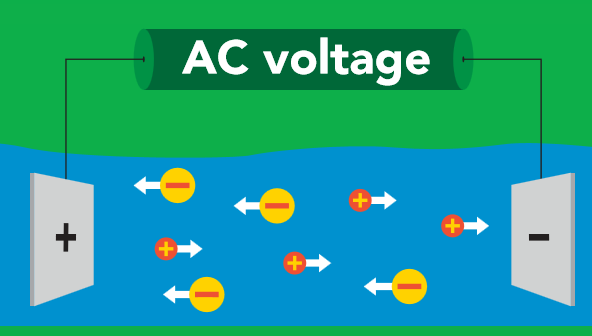
\includegraphics[width=90mm, height=60mm]{Imagenes/2021/imag37.png}
    \caption[Principio de Funcionamiento del Sensor de Conductividad]{Principio de Funcionamiento del Sensor de Conductividad. \textbf{Fuente: }\cite{ezoce}.}
    \label{fig:4.14}
\end{figure}

En la Tabla \ref{tab:caract_ce} se muestran las principales características del sensor de conductividad.
Entre los usos comunes de este sensor se encuentran el uso estándar en laboratorio, uso en el campo, en acuaponía, hidroponía y en acuarios.
\begin{table}[H]
\protect\caption[Características del sensor de CE de AtlasScientific]{Características del sensor de CE de AtlasScientific.}
\label{tab:caract_ce}
\begin{center}
\begin{tabular}{|l|l|}
\hline
Rango    &  5 - 200.000 $\mu S\/cm$\\
\hline
Exactitud      &  +/-2\% \\
\hline
Conector &  BNC macho\\
\hline
Resolución   &  +/-0.0001\\
\hline
Tiempo de Respuesta   &  90\% en 1s\\
\hline
Presión Máxima    &  3,447 kPa (500 PSI) \\
\hline
Profundidad Máxima	& 343 metros\\
\hline
Rango de Temperatura $^{\circ}$C	& 1- 110\\
\hline
Longitud del Cable	& 1m\\
\hline
Sensor de Temperatura Interno	& NO\\
\hline
Tiempo antes de recalibración	& 10 año\\
\hline
Tiempo de Vida	& aprox. 10 años\\
\hline
Dimensiones	& 12mm x 152mm\\
\hline
Peso	& 51 gramos\\
\hline
Superficie de medición	& Grafito\\
\hline
Seguro en Alimentos	& Si\\
\hline
\end{tabular}
\vspace{5mm}
\newline
\hfill \textbf{Fuente:} \cite{atlasce}
\end{center}
\end{table}

%%%%%%%%%%%%%%%%%%%%%%%%CAMBIAR
\subparagraph{Sensor de Temperatura}
En la Figura \ref{fig:4.15}  se puede apreciar el sensor de Temperatura utilizado fabricado por la empresa Atlas Scientific.


\begin{figure}[t]
    \centering
    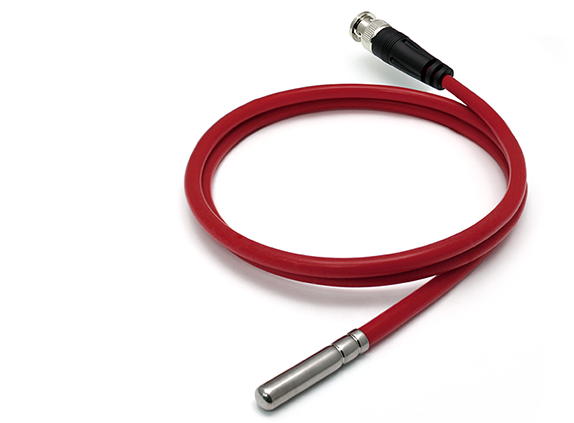
\includegraphics[width=90mm, height=70mm]{Imagenes/2021/imag39.png}
    \caption[Sensor de Temperatura PT 1000]{Sensor de Temperatura PT 1000. \textbf{Fuente: } Página Web del Fabricante. }
    \label{fig:4.15}
\end{figure}


\textbf{Principio de Operación: }
A diferencia de cualquier otro material, la correlación entre la resistencia y la temperatura en el platino es bastante lineal. Es por esta razón que el sensor de temperatura RTD de platino es el estándar industrial para la medición de temperatura.

La sonda de temperatura PT-1000 es un termómetro tipo resistencia. Donde PT significa platino y 1000 es la resistencia medida de la sonda a 0$^{\circ}$C en $\Omega$ (1k a 0$^{\circ}$C).
A medida que la temperatura cambia, la resistencia del platino cambia.
Para convertir la resistencia de la sonda a la temperatura, se utiliza la siguiente ecuación simplificada

\begin{equation}
    T=-\frac{\sqrt{(-0.00232(R)+17.59246)}-3.908}{0.00116}
\end{equation}

Donde $T$ esta en grados Celsius y $R$ es el valor de la resistencia medida por el sensor.

El módulo utilizado para el tratamiento de las señales es el mostrado en la Figura \ref{fig:4.16} también fabricado por la empresa Atlas Scientific.

\begin{figure}[t]
    \centering
    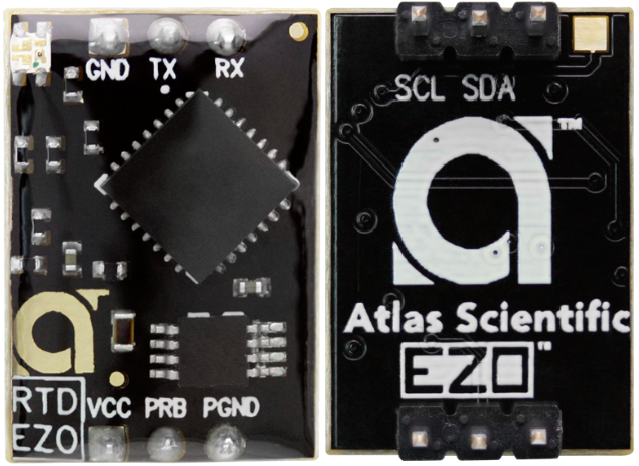
\includegraphics[width=90mm, height=70mm]{Imagenes/2021/imag38.png}
    \caption[EZO-RTD Circuito Integrado de Temperatura]{EZO-RTD Circuito Integrado de Temperatura.\textbf{Fuente: }Pagina Web del Fabricante.}
    \label{fig:4.16}
\end{figure}

Es un sistema informático de tamaño reducido que está diseñado específicamente para ser utilizado en aplicaciones donde se requiera mediciones exactas y precisas de la temperatura a través de una sonda de temperatura genérica PT-100 / PT-1000. Se conecta directamente a la placa Tentacle T3 y no necesita de aislamiento a diferencia de los otros módulos de sensores.

En la Tabla \ref{tab:caract_temp} se visualizan las características del Sensor de Temperatura PT-1000.
Entre las aplicaciones de uso común de este sensor están el uso estándar de laboratorio, uso en el campo, en el suelo, acuapon\'ia, hidroponía, en bebidas como cerveza, vino u otro licor.

% Sensor REDOX
% Sensor OD


\textbf{Bloque de Control}
Este bloque es el encargado de realizar el procesamiento de los datos recibidos a través de los sensores y la configuración de parámetros adquirida por la Interfaz de Usuario.

\begin{itemize}
    \item \textbf{Hardware:}
    En la Figura \ref{fig:4.4} se observa la placa de desarrollo low cost escogida para el presente proyecto, la Raspberry Pi 3 model B desarrollado por la fundación Raspberry Pi. La misma cuenta con un procesador multimedia Broadcom BCM2835 system-on-chip (SoC).
    \newline
    \hfill
    La CPU Contiene un ARM1176JZFS, con unidad de coma flotante, que funciona a 700Mhz y es capaz de soportar overclock a 1GHZ en modo “TURBO” que hace que el SoC de más rendimiento sin reducir el tiempo de vida de la placa y sin perder la garantía. 
    La memoria RAM es de 512MB de SDRAM (en su modelo B), en un único módulo, el cual, funciona a 400Mhz en su modo normal y alcanzando los 600Mhz en su versión “TURBO”.
    La  Raspberry Pi no tiene un disco duro tradicional, para ello dispone de un lector para memorias SD, un sistema de almacenamiento en estado sólido. El arranque del sistema se hará desde la propia tarjeta SD, con lo que, debido a que tiene que albergar todo el sistema operativo, es necesario que la tarjeta sea de al menos 2 GB de capacidad para almacenar todos los archivos requeridos.
    La placa carece de botón de encendido y apagado, con lo que la energía le llega mediante un conector microUSB estándar de 5V. El consumo de la placa es de 700mA, (3,5W).
    La Raspberry Pi, está diseñada para ejecutar el sistema operativo GNU/Linux y la version mas extendido es el Raspberry Pi OS .
    \begin{figure}[t]
        \centering
        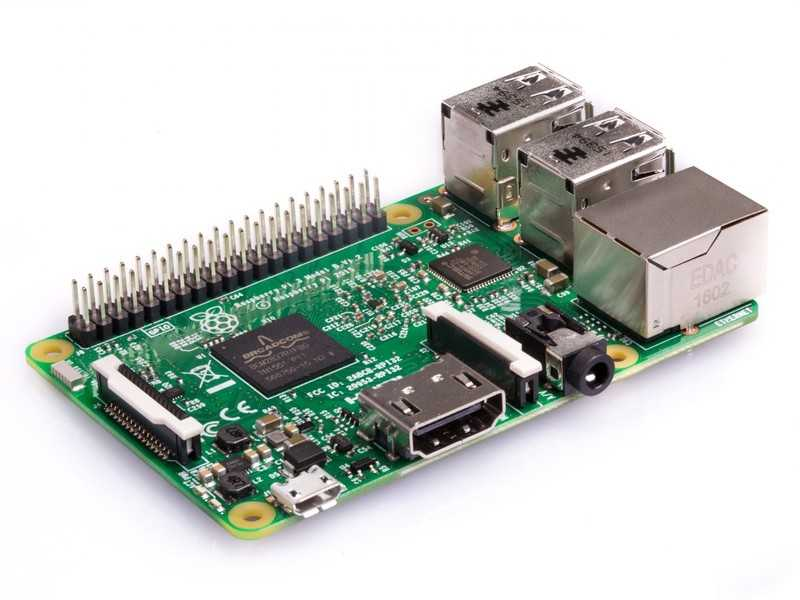
\includegraphics[width=100mm, height=70mm]{Imagenes/2021/imag35.jpg}
        \caption[Placa Raspberry Pi 3 model B]{Placa Raspberry Pi 3 model B.\textbf{Fuente:} Página Web del Fabricante.}
        \label{fig:4.4}
    \end{figure}

    Se optó por este controlador por sus prestaciones,  t\'ecnicas, suficientes para las tareas a ser ejecutadas, con un almacenamiento externa de 64 Gb con una memoria tipo microSD de alto rendimiento, por sus dimensiones reducidas, la raspberry  eran acorde a los requerimientos necesarios y por tener un gran soporte y comunidad activa en l\'inea.
 
    En la Tabla \ref{tab:carac_rasp} se detallan las principales características técnicas de la Raspberry Pi 3 model B.
 
 \begin{table}[t]
      \protect\caption[Características Técnicas. Raspberry Pi 3 model B]{Características Técnicas. Raspberry Pi 3 model B.  \label{tab:carac_rasp}}
    
     \centering
     \begin{tabular}{l c}
        \toprule
           Sistema Operativo & Raspberry Pi OS\\
%          \hline
          Juego de Instrucciones & RISC 64 bits\\
%          \hline
          Procesador & RQuad Core 1.2GHz Broadcom BCM2837\\
%          \hline
          RAM  & 1 GB\\
%          \hline
          Bluetooth &  4.2 Low Energy (BLE)\\
%          \hline
          Puertos USB 2.0 & 4\\
%          \hline
          GPIO& 40\\
%          \hline
          UART& 2\\
%          \hline
          I2C& 4\\
%          \hline
          Stero/Video & 1\\
%          \hline
          HDMI & 1\\
%          \hline
          CSI(RPI Camera) & 1\\
%          \hline
          DSI(RSP Touchscreen display) & 1\\
%          \hline
          Dimensiones & 85.60 mm x 53.98 mm\\
%          \hline
          Peso & 50 g\\
%          \hline
          Consumo energ\'etico & 4 W\\
%          \hline
          Alimentaci\'on & 5 V\\
%          \hline
     \bottomrule   
     \end{tabular}
     \vspace{5mm}
     \newline
     \hfill \textbf{Fuente:} Elaboración Propia. Información recopilada de \cite{rasp}
\end{table}
    Por otra parte, para eliminar la necesidad de cableado, multiplexación y aislamiento eléctrico en la lectura de los sensores, se optó por la utilización de la placa open source Tentacle Shield para arduino de Whitebox labs, la cual se muestra en la Figura \ref{fig:4.5}.
\begin{figure}[t]
    \centering
    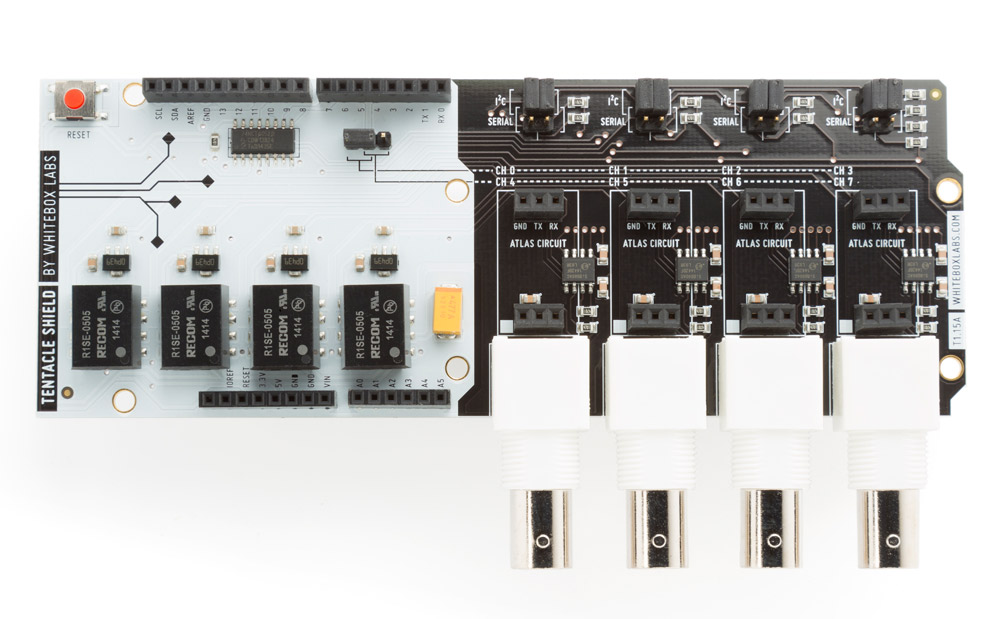
\includegraphics[width=100mm, height=70mm]{{Imagenes/2021/imag26.jpg}}
    \caption[Placa Tentacle para Arduino]{Placa Tentacle para Arduino. \textbf{Fuente:} Página web del Fabricante}
    \label{fig:4.5}
\end{figure}

    Es una forma pr\'actica y fácil de leer múltiples sensores de la empresa Atlas Scientific, la placa puede alojar hasta 4 dispositivos EZO de Atlas Scientific para medir pH(Potencial de Hidrógeno), Oxígeno Disuelto(DO por sus siglas en inglés), conductividad eléctrica(CE), Temperatura(T), Potencial de Reducción de Oxidación(ORP por sus siglas en inglés)

    \textbf{Aislamiento:}
    Los circuitos de medición y las líneas de comunicación aislados individualmente evitan el ruido y los bucles de tierra para obtener mediciones precisas, incluso en sistemas de bucle cerrado.Los sensores no interferirán entre sí y la mayoría del ruido eléctrico exterior que puede interferir con las lecturas se reducirá.

    \item \textbf{Software:}El software de control fue desarrollado en el lenguaje de programación Python. Este es un lenguaje interpretado multiparadigma, soporta programación orientada a objetos, imperativa y funcional.
    Python ya viene instalado en el sistema operativo Raspberry Pi OS para Raspberry Pi.Tiene la ventaja de poder utilizar los pines GPIO de la placa de desarrollo para conectar el mundo digital con el mundo físico mediante la programación, facilitando de esta manera el control de la lectura de los distintos sensores y el accionamiento de los actuadores utilizados.
    
    El administrador de Base de Datos utilizado fue Sqlite3, es un sistema de gestión de base de datos ampliamente difundido en el mundo de la programación de aplicaciones móviles.
    La utilización de este gestor fue debido a su gran portabilidad y su capacidad  de gestionar bases de datos de hasta 2 terabyte de tamaño.
    En la Tabla \ref{tab:caract_sqlite} se muestran las características más relevantes de la Base de Datos Sqlite.

    \begin{table}[H]
    \protect\caption[Características del Gestor de Base de Datos SQLITE]{Características del Gestor de Base de Datos SQLITE.\label{tab:caract_sqlite}}
        \centering
        \begin{tabular}{|l|l|}
            \hline
            Soporte & Múltiples tablas,\textit{triggers} y vistas   \\
            \hline
             Lectura y Escritura& \multicolumn{1}{|l|}{\begin{tabular}[c]{@{}l@{}}  Directamente sobre archivos que se encuentran en el disco \\ duro.\end{tabular}} 
             \\
             \hline
             Formato & 
             \multicolumn{1}{|l|}{\begin{tabular}[c]{@{}l@{}}  Multiplataforma. Puede ser utilizado en sistemas de 32 bits \\ o 64 bits.\end{tabular}} 
           \\
             \hline
             Operaciones &\multicolumn{1}{|l|}{\begin{tabular}[c]{@{}l@{}} Realiza operaciones de manera más eficiente y rápido que  \\ MySql y PostgreSQL.\end{tabular}} 
            \\
             \hline
             Interfaz API &\multicolumn{1}{|l|}{\begin{tabular}[c]{@{}l@{}}Opera con diversas Interfaces API lo que permite trabajar  \\con C++, PHP, Python, Groovy, etc.\end{tabular}} 
            \\
             \hline
             Dependencias Externas & No\\
             \hline
             Librerías & Cuentan con acceso para muchos lenguajes de programación.\\
             \hline
             UDF & Soporta funciones SQL definidas por el usuario.\\
             \hline
             Código Fuente & Dominio público y documentación extensa.\\
             \hline
        
        \end{tabular}
        \vspace{5mm}
        \newline
        \hfill \textbf{Fuente: }P\'agina Web del desarrollador.\cite{sqlite}
        
    \end{table}
    
\end{itemize}
%%%%%%%%%%%%%%%%%%%%%%%%%%%%%%%%%%%%
\subsubsection[Batimetr\'ia]{Batimetr\'ia}
\subsubsection[Gr\'ua ]{Gr\'ua}


\subsection[Dise\~no Control]{Dise\~no Control}
\subsubsection[Sonda]{Sonda}
\begin{table}[t]
\protect\caption[Funciones Generales]{Funciones Generales. \label{tab:fun_general}}
    \centering
    \begin{tabular}{l l l}
        \toprule
        \textbf{Descripción} & \textbf{Decisión} & \textbf{Característica} \\
        \midrule
         Comunicaci\'on  Perif\'ericos  & Algoritmo comunicaci\'on & \multicolumn{1}{ l}{\begin{tabular}[c]{@{}l@{}} Env\'io y recipci\'oon de estados \\ funcionamiento y datos de los \\ dispositivos conectados a la red \end{tabular}}
         \\
%        \hline
        Lectura de Sensores & Algoritmo muestreo & \multicolumn{1}{l}{\begin{tabular}[c]{@{}l@{}} Se Lectura secuencial de los\\ sensores pH, CE,\\ OD, OPR, T\end{tabular}}
         \\
%        \hline
        Almacenamiento datos & Algoritmo datos &
        \multicolumn{1}{l}{\begin{tabular}[c]{@{}l@{}} Consulta y registro as\'incrono \\ 
        del muestreo\end{tabular}}
         \\
%        \hline
        Transmisi\'on datos  & Algoritmo transmisi\'on &
        \multicolumn{1}{l}{\begin{tabular}[c]{@{}l@{}} Transmisi\'on asincr\'onica \\ a estaci\'on remota \end{tabular}}
           \\
        \bottomrule
    \end{tabular}
    \vspace{5mm}
    \newline
    \hfill \textbf{Fuente:} Elaboración Propia
\end{table}
\section{Descripci\'on  sistema }
\section[Descripción General del Sistema]{Descripción General del Sistema}
En referencia al modelo conceptual del sistema, este está constituido, por un bloque interfaz de usuario, un bloque de control, un bloque de sensores, un bloque de actuadores y un bloque de alimentaci\'on,  como se puede apreciar en la Figura \ref{fig:4.1}.
\section[Características Técnicas de los módulos]{Características Técnicas del módulo Despliegue}
La Tabla \ref{tab:carac_general} detalla las características técnicas del mecanismo a ser desarrollado, teniendo en cuenta los objetivos planteados en la Sección 1.3.
\begin{table}[H]
\protect\caption[Datos T\'ecnicos]{Datos T\'ecnicos. \label{tab:carac_general}}
    \centering
    \scalebox{0.9}{\begin{tabular}{|c|c|}
        \hline
        \textbf{Caracter\'istica} & \textbf{Valor}  \\
        \hline
        \multicolumn{2}{|c|}{\textbf{F\'isico}} \\
        \hline
        Capacidad de carga & $ > 10 [Kg] $   \\
        \hline
        Dimensiones & $< 50 [cm]$  x $50 [cm]$ x $50 [cm]$    \\
        \hline
        Peso &  $ < 15 kg$ \\
        \hline
        Caja Electr\'onica & Herm\'etica  \\
        \hline
        \multicolumn{2}{|c|}{\textbf{Eléctrico}} \\
        \hline
         Alimentaci\'on & 12 V DC  \\
        \hline
         Autonom\'ia & No  \\
        \hline
         \multicolumn{2}{|c|}{\textbf{Interfaz}} \\
         \hline
         Configuraci\'on de Par\'ametros & Por Interfaz Gr\'afica  \\
        \hline
         Transmisi\'on Remota  & Si  \\
        \hline
    \end{tabular}}
    \vspace{5mm}
    \newline
    \hfill \textbf{Fuente:} Elaboraci\'on Propia
\end{table}
\subsubsection[Batimetr\'ia]{Batimetr\'ia}
\subsubsection[Gr\'ua ]{Gr\'ua}


\subsection[Dise\~no de Interfaz]{Dise\~no de Interfaz}
\subsubsection[Sonda]{Sonda}
\subsubsection[Batimetr\'ia]{Batimetr\'ia}
\subsubsection[Gr\'ua ]{Gr\'ua}


\section[Fabricaci\'on]{Fabricaci\'on}
\subsubsection[Sonda]{Sonda}
La fabricaci\'on de las partes de la sonda se realiz\'o con dos t\'ecnicas desarrollados en el cap\'itulo anterior, la base y el anillo se realizaron con la t\'ecnica de fabricaci\'on sustractiva de   se realiz\'o en el laboratorio de Metal Mec\'anica de la Facultad de Ingenier\'ia Universidad Nacional de Asunci\'on, con un torno semiatom\'atico, con la t\'ecncia de vaciado progresivo. 
        
\begin{figure}[h]
\centering
\fbox{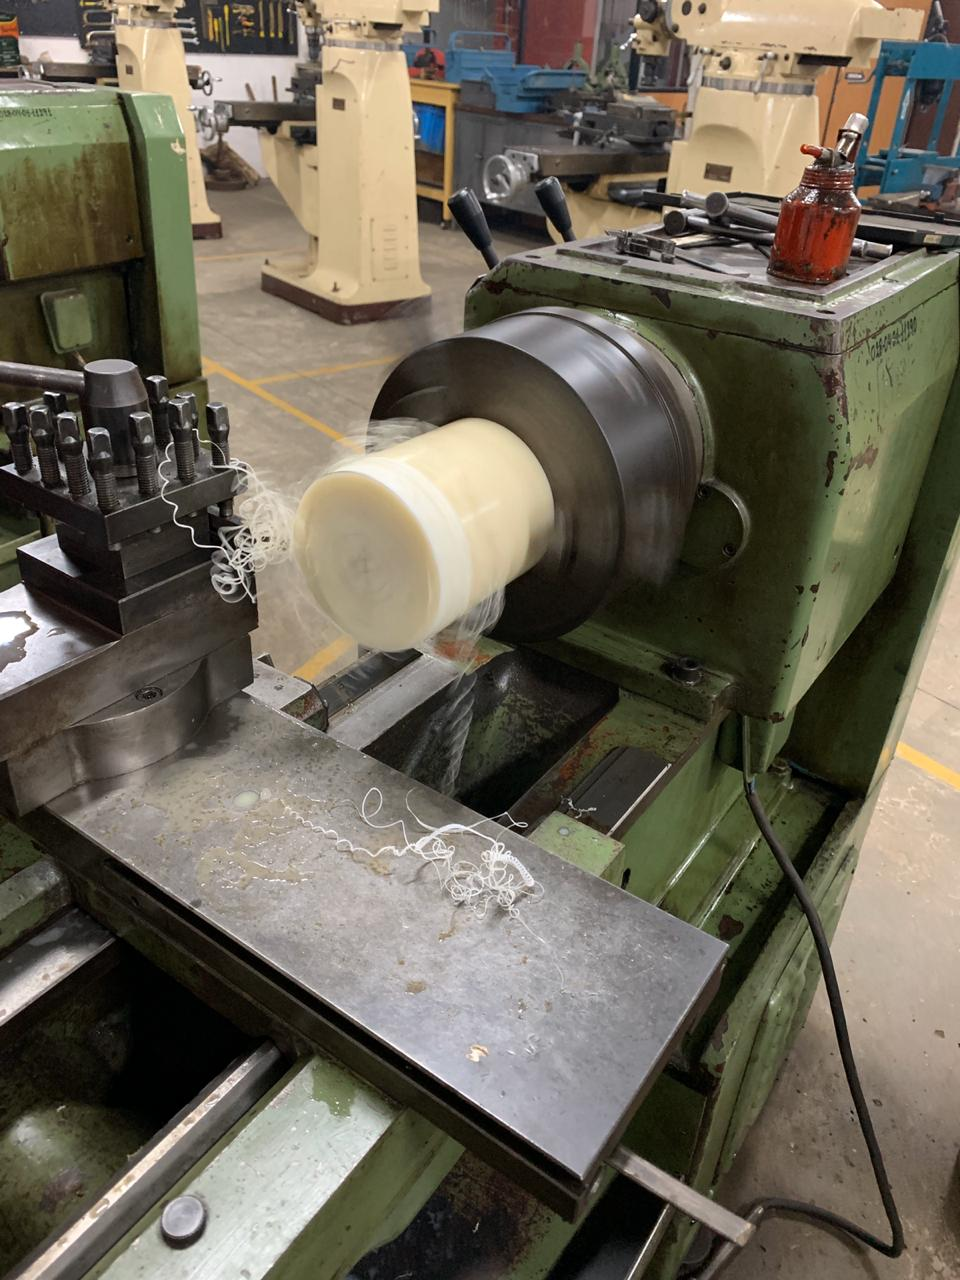
\includegraphics[scale=0.2]{Imagenes/2019/Sonda_Fab0.jpeg} }
\caption{Tubo de Nylon r\'igido en proceso de desgaste. Fuente: elaboración propia}
\label{fig:preparacion}
\end{figure}
 
\hfill\section{Fabricaci\'on de la Sonda.}
\begin{figure}[t]
\centering
\fbox{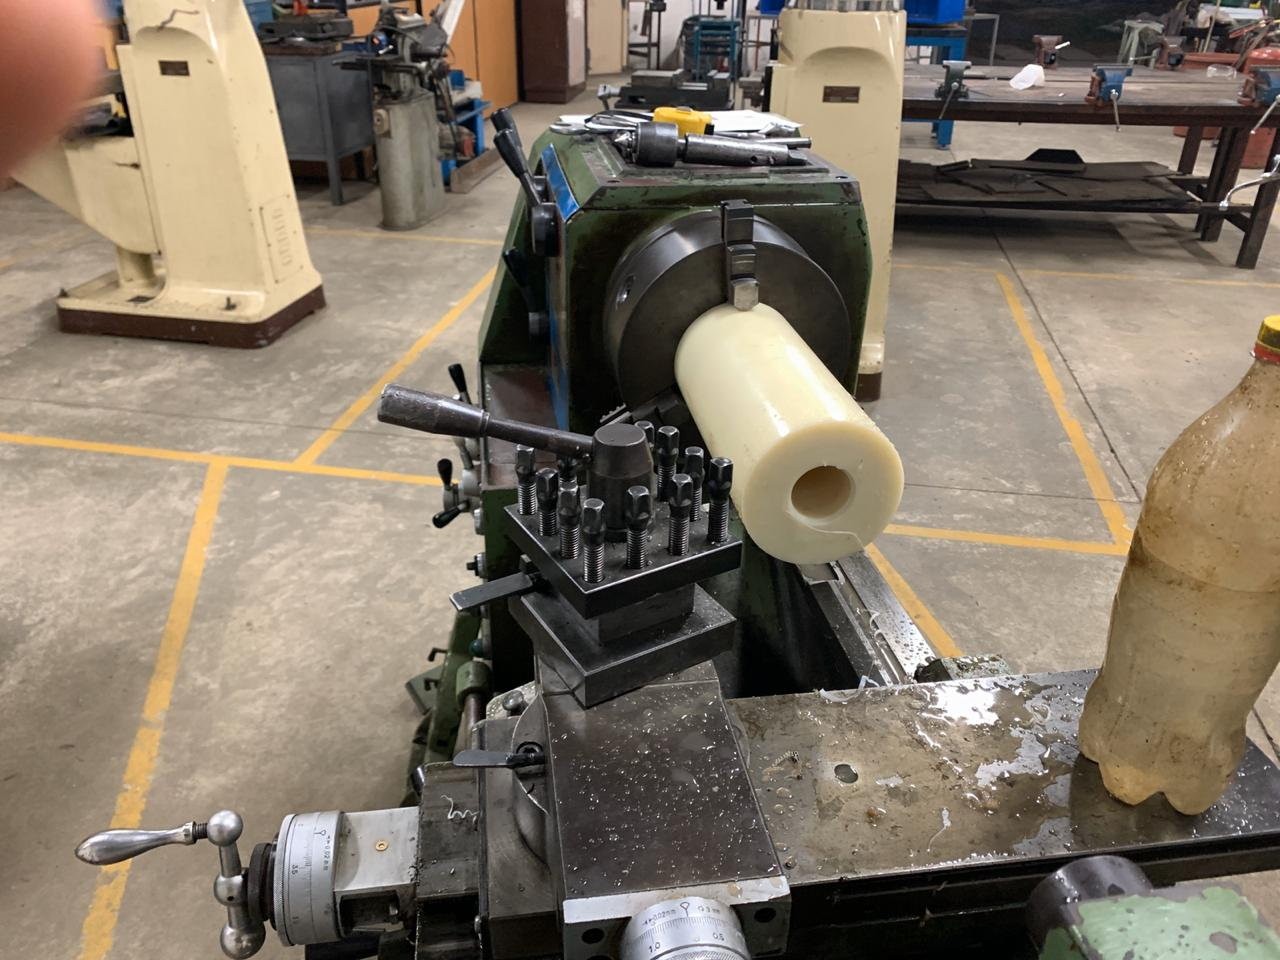
\includegraphics[scale=0.2]{Imagenes/2019/Sonda_Fab.jpeg}}
\caption{Tubo de Nylon r\'igido, proceso de vaciado. Fuente: elaboración propia}
\label{fig:preparacion}
\end{figure}

\subsubsection[batimetría]{Batimetr\'ia} 
Tal como se observa en la figura \ref{fig:batimetro} el sistema de medici\'on de profundidad fue dise\~nado de tal forma que permita ser instalado en la parte posterior (popa) del VAS, mediante dos abrazaderas, uno de su sujeci\'on y otra de sujeci\'on - nivelaci\'on para asegurarse  pueda estar en contacto con el agua al momento de instalarse.  Para la correcta  instalci\'on de se debe alinear el sonar con la parte m\'as baja de la popa 

\begin{figure}[h]
\centering
\fbox{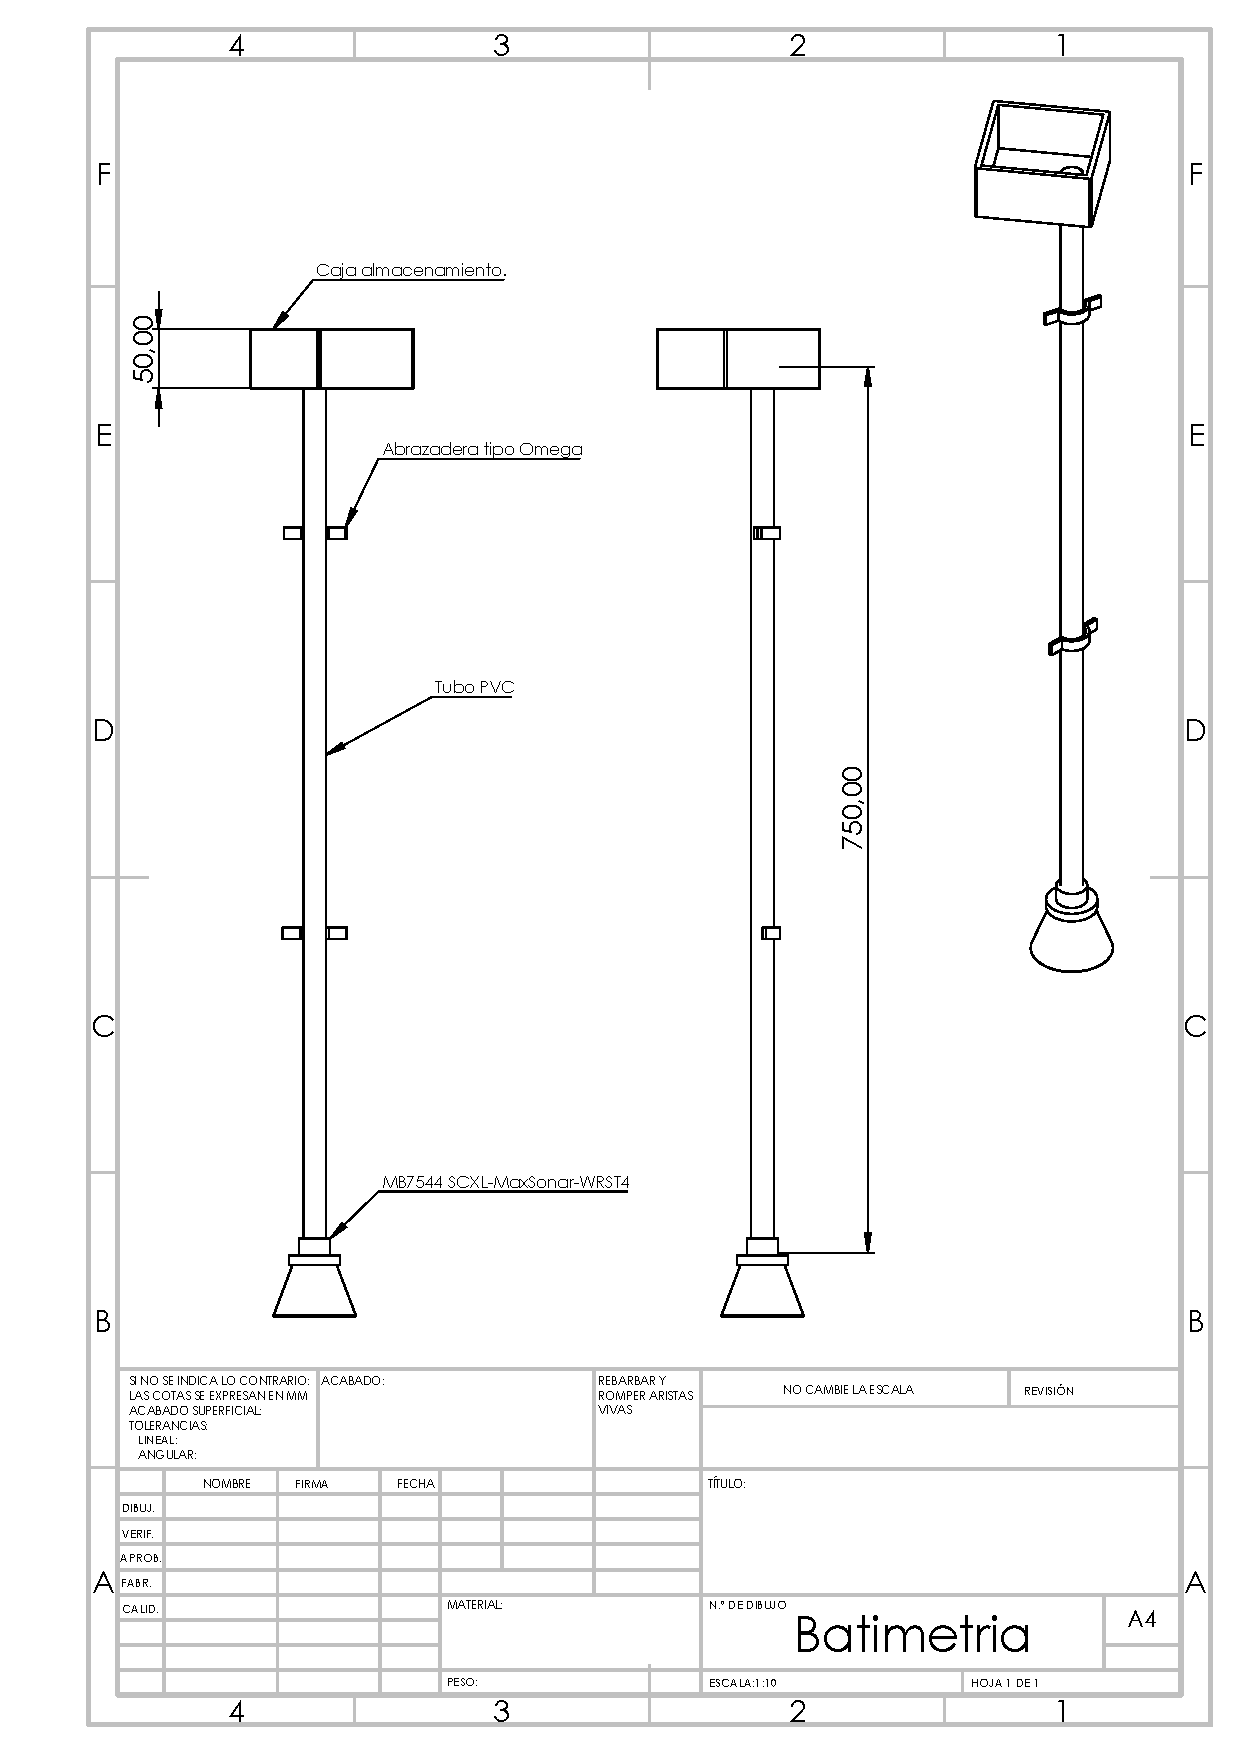
\includegraphics[scale=0.6]{Imagenes/cap3/Batimetria.pdf}}
\caption{Dise\~no final de medidor de profundidad. \textbf{Fuente:} elaboración propia}
\label{fig:batimetro}
\end{figure}

para estructura del sistema de batimetr\'ia tubos de PVC (Policloruro de Vinilo) roscables para la construcci\'on de la estructura de soporte, la secci\'on m\'as larga tiene una longitud de 1,5 [m], con el objetivo de poder ajustar la distancia de medici\'on inicial y que el sonar ubicado en el extremo est\'e totalmente sumergido. El sistema de fijaci\'on y ajuste est\'a compuesta por dos abrazaderas, una del tipo omega utilizada como gu\'ia de desplazamiento y la otra de abrazadora tipo "O" para el ajuste de profundidad. 


\subsubsection[Gr\'ua ]{Gr\'ua}
